\section{Fused Sparse Decode Attention}
\label{sec:decode}

\begin{figure}[t]
  \centering
  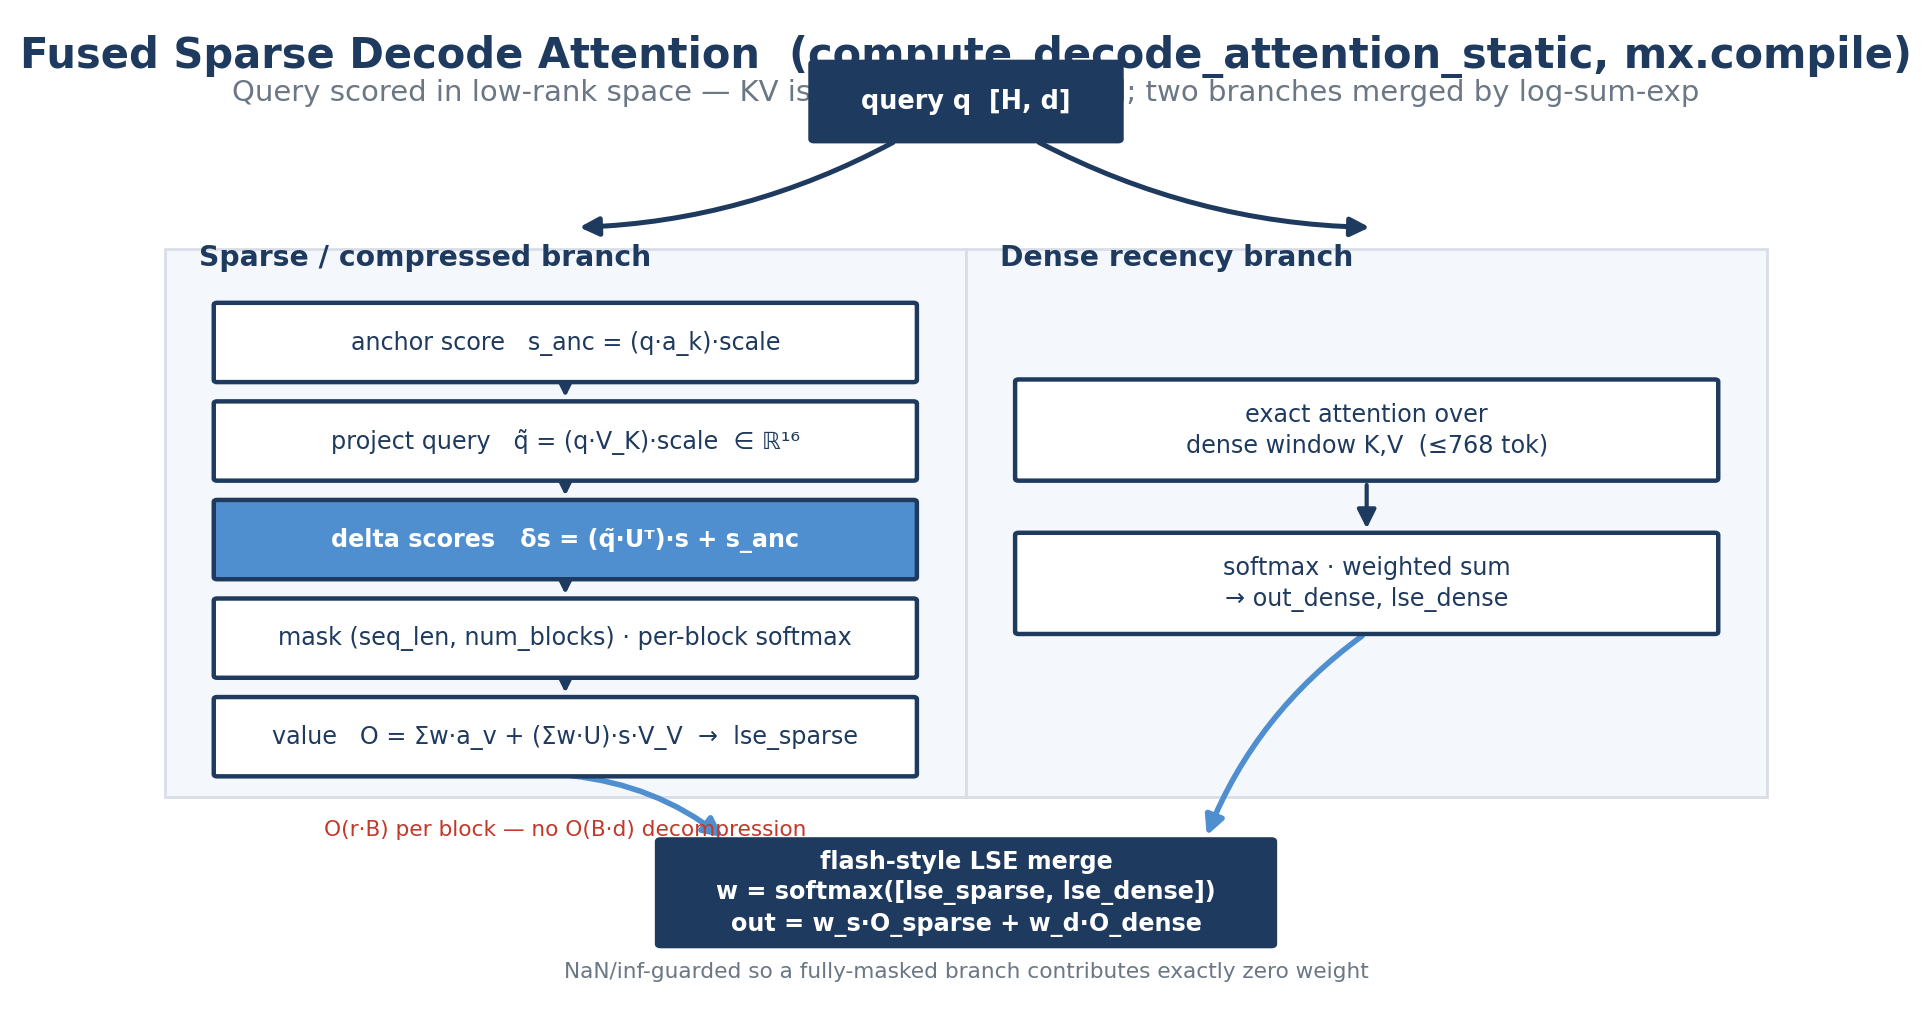
\includegraphics[width=\linewidth]{figures/f5_decode_attention.png}
  \caption{The fused decode kernel. The query is scored against every compressed block
  \emph{in low-rank coordinates}---projected through each block's basis rather than against
  reconstructed keys---and against the dense recency window; the two branches are merged by a
  numerically stable log-sum-exp. The entire computation is one \texttt{mx.compile}-d Metal
  graph and never reconstructs dense KV.}
  \label{fig:decode}
\end{figure}

The decode kernel (\texttt{compute\_decode\_attention\_static}, a single
\texttt{mx.compile}-d function) is where the compressed representation has to pay for itself:
it must produce the same attention output a dense cache would, reading only the factors from
\S\ref{sec:compression}. It has a compressed branch, a dense branch, and a stable merge
(Fig.~\ref{fig:decode}, Alg.~\ref{alg:decode}). Let $q\in\R^{H\times\dhead}$ be the current
query (group-query attention replicates the $\Hkv$ KV heads to the $H$ query heads), and let
$\sigma$ be the attention scale.

\subsection{Scoring in low-rank space}
The key observation is that the score of $q$ against a reconstructed key
(Eq.~\ref{eq:recon}) factors through the basis, so we never form the key. Against block $b$:
\begin{align}
\text{(anchor)}\quad & s^{\text{anc}}_b = \sigma\, \langle q,\ \anchork^{(b)}\rangle,\\
\text{(project)}\quad & \tilde q_b = \sigma\, q\, V_K^{(b)} \in\R^{\rank},\\
\text{(deltas)}\quad & \delta s_b = s_b\,\big(\tilde q_b\, U_b^{\!\top}\big) + s^{\text{anc}}_b
 \in\R^{S}.
\end{align}
The middle step projects the query into the block's $\rank$-dimensional key subspace once; the
third recovers the per-token delta scores by a single $\rank{\times}S$ product. The cost is
$O(\Hkv\rank\dhead + \rank S)$ per block---\emph{independent of reconstructing the
$S{\times}\dhead$ keys}, the central efficiency of the design. Tokens beyond a block's valid
length and slots beyond the live block count are masked to $-\infty$. Per-block scores
$[s^{\text{anc}}_b,\delta s_{b,1},\dots,\delta s_{b,S}]$ are gathered across all blocks; a
softmax over the whole compressed set yields weights $w$ and a log-sum-exp
$\ell^{\text{sp}}$.

\subsection{Reconstructing the output without decompression}
The attention output over the compressed set is likewise assembled from the factors. Writing
$w^{\text{anc}}_b$ and $w^{d}_b\in\R^{S}$ for a block's anchor and delta weights,
\begin{equation}
O = \underbrace{\sum_b \big(w^{\text{anc}}_b + \textstyle\sum_i w^{d}_{b,i}\big)\,\anchorv^{(b)}}_{\text{anchor value mass}}
 \;+\; \underbrace{\sum_b s_b\,\big(w^{d}_b\, U_b\big)\,V_V^{(b)}}_{\text{delta value mass}},
\end{equation}
where the delta term contracts the weights through the same $U$ used for scoring and then
through the value basis $V_V$---again never forming dense values. The result is the compressed
branch output $O^{\text{sp}}$ with its log-sum-exp $\ell^{\text{sp}}$.

\subsection{Dense branch and stable merge}
The dense branch is exact attention over the recency window, giving $O^{\text{dn}}$ and
$\ell^{\text{dn}}$. The two are combined as a two-way flash-style reduction:
\begin{equation}
m=\max(\ell^{\text{sp}},\ell^{\text{dn}}),\quad
O = \frac{e^{\ell^{\text{sp}}-m}O^{\text{sp}} + e^{\ell^{\text{dn}}-m}O^{\text{dn}}}
        {e^{\ell^{\text{sp}}-m} + e^{\ell^{\text{dn}}-m}}.
\end{equation}
This is the standard log-sum-exp combination of two softmax partitions, and it is correct only
if a \emph{fully masked} branch contributes exactly zero weight. When there are no compressed
blocks yet, every compressed score is $-\infty$, so $\ell^{\text{sp}}=-\infty$ and the naive
softmax produces NaNs that, left unguarded, propagate through $o_{\text{proj}}$ into the next
layer's query. The kernel therefore sanitizes each branch's log-sum-exp and output to a
finite, fully-down-weighted value before the merge---a guard the source documents as a real
bug fix, and one we retain verbatim.

\begin{algorithm}[t]
\caption{\textsc{FusedDecodeAttention} (one token, one layer)}
\label{alg:decode}
\begin{algorithmic}[1]
\Require query $q$; pool $\{U,V_K,V_V,\anchork,\anchorv,s,\ell\}_{1:n}$; window $K^{\text{win}},V^{\text{win}}$
\For{each block $b$}
  \State $s^{\text{anc}}_b\gets\sigma\langle q,\anchork^{(b)}\rangle$;\ \ $\tilde q_b\gets\sigma\,qV_K^{(b)}$
  \State $\delta s_b\gets s_b(\tilde q_b U_b^{\!\top})+s^{\text{anc}}_b$;\ mask invalid tokens/slots
\EndFor
\State $w\gets\softmax(\text{all block scores})$;\ \ $\ell^{\text{sp}}\gets\lse(\cdot)$
\State $O^{\text{sp}}\gets \sum_b(w^{\text{anc}}_b{+}\!\sum_i w^{d}_{b,i})\anchorv^{(b)} + \sum_b s_b(w^d_b U_b)V_V^{(b)}$
\State $O^{\text{dn}},\ell^{\text{dn}}\gets \textsc{ExactAttn}(q,K^{\text{win}},V^{\text{win}})$
\State sanitize NaN/$\infty$ in $(\ell^{\text{sp}},\ell^{\text{dn}},O^{\text{sp}},O^{\text{dn}})$
\State \Return flash-merge$(O^{\text{sp}},\ell^{\text{sp}},O^{\text{dn}},\ell^{\text{dn}})$
\end{algorithmic}
\end{algorithm}

\subsection{Compute profile}
Per token the kernel does $O\!\big(n(\Hkv\rank\dhead+\rank\bs)\big)$ work for $n$ compressed
blocks plus $O(\Hkv\dwin\dhead)$ for the window. Two properties follow. First, the work is
linear in the number of \emph{blocks} ($n=N/\bs$), not tokens, with a small $\rank$-weighted
constant---asymptotically attractive. Second, the constant is realized through many small
tensor ops inside one compiled graph, and on the test hardware these do not yet match the
throughput of MLX's native fused attention over a contiguous cache; \S\ref{sec:eval}
quantifies the resulting decode-throughput gap, and \S\ref{sec:limitations} discusses why a
hand-written fused kernel (e.g. CUDA/Triton or a custom Metal op) is the natural next step.
